\documentclass{article}
\usepackage[utf8]{inputenc}
\usepackage[english]{babel}

% Convenience improvements
\usepackage{csquotes}
\usepackage{enumitem}
\setlist[enumerate,1]{label={\alph*)}}
\usepackage{amsmath}
\usepackage{amssymb}
\usepackage{mathtools}
\usepackage{tabularx}

% Proper tables and centering for overfull ones
\usepackage{booktabs}
\usepackage{adjustbox}

% Change page/text dimensions, the package defaults work fine
\usepackage{geometry}

\usepackage{parskip}

% Drawings
\usepackage{tikz}
\usepackage{forest}

% Adjust header and footer
\usepackage{fancyhdr}
\pagestyle{fancy}
\fancyhead[L]{Embedded \& Pervasive Systems --- \textbf{Workshop 1}}
\fancyhead[R]{}
\fancyfoot[C]{}
\fancyfoot[R]{\thepage}
% Stop fancyhdr complaints
\setlength{\headheight}{12.5pt}

\newcommand{\Deltaop}{\, \Delta\, }
\newcommand{\xor}{\, \oplus\, }

\begin{document}

\begin{enumerate}[label={\arabic*.}]
    \item \textbf{Motion Sensing}
    \begin{enumerate}
        \item We expect the x and y values to be close to zero and z to be close to 1. This is because the accelerometer is at rest, but affected by gravity.
        
        \item We expected the accelerometer values to be more steady, considering that it did not visibly move during the time we sampled the values.

        \begin{verbatim}
time, acc x, acc y, acc z, gyr x, gyr y, gyr z, mag x, mag y, mag z
1710510287225, 0.01, 0.09, 0.94, 0.00, 0.00, 0.00, -9.76, -27.29, 16.92
1710510287765, -0.01, -0.00, 0.97, 0.03, -0.05, 0.01, -15.39, -44.25, 26.25
1710510288307, 0.06, 0.02, 0.96, 0.05, -0.08, 0.01, -16.91, -52.01, 31.04
1710510288846, 0.05, 0.01, 0.97, -0.06, 0.09, -0.01, -17.94, -56.20, 33.49
1710510289389, 0.08, 0.02, 0.95, -0.08, 0.12, -0.02, -17.58, -57.48, 34.31
1710510289928, 0.13, 0.05, 1.01, 0.10, -0.12, 0.08, -16.54, -57.01, 35.34
1710510290471, 0.27, 0.13, 0.97, 0.04, -0.50, -0.13, -13.15, -53.37, 33.13
1710510291017, 0.33, 0.11, 0.86, 0.13, -0.08, 0.06, -8.03, -49.43, 29.82
1710510291560, 0.38, 0.09, 0.85, -0.07, 0.17, 0.00, -5.01, -47.85, 27.32
1710510292103, 0.35, 0.10, 0.91, -0.05, -0.04, 0.04, -3.89, -47.59, 26.18
        \end{verbatim}

        \item We assume that some instability is caused by slight inaccuracies of the sensors. In the case of the magnetometer they might also be distorted by nearby magnetic fields. (Although we are not sure how plausible that is.)
        
        Depending on the requirements, this could be resolved for example by \begin{itemize}
            \item requiring an (absolute) sensor value change of more than some threshold compared to the current value before updating the current value
            \item taking new values as points of evidence, not fact, and slowly adjusting current values if the points of evidence agree (\enquote{Bayesian-like} smoothing, perhaps with some interpolation between points of evidence)
        \end{itemize}
    \end{enumerate}

    \item \textbf{Applications of Motion Sensing}
    \begin{enumerate}
        \item If the z value of the accelerometer is below some threshold (to be determined experimentally) then we consider the sensor to be falling.
        
        Such a check would have to be added to the main loop.

        \item The shake is clearly identifiable in Figure \ref{fig:shake1}.
        \begin{figure}
            \centering
            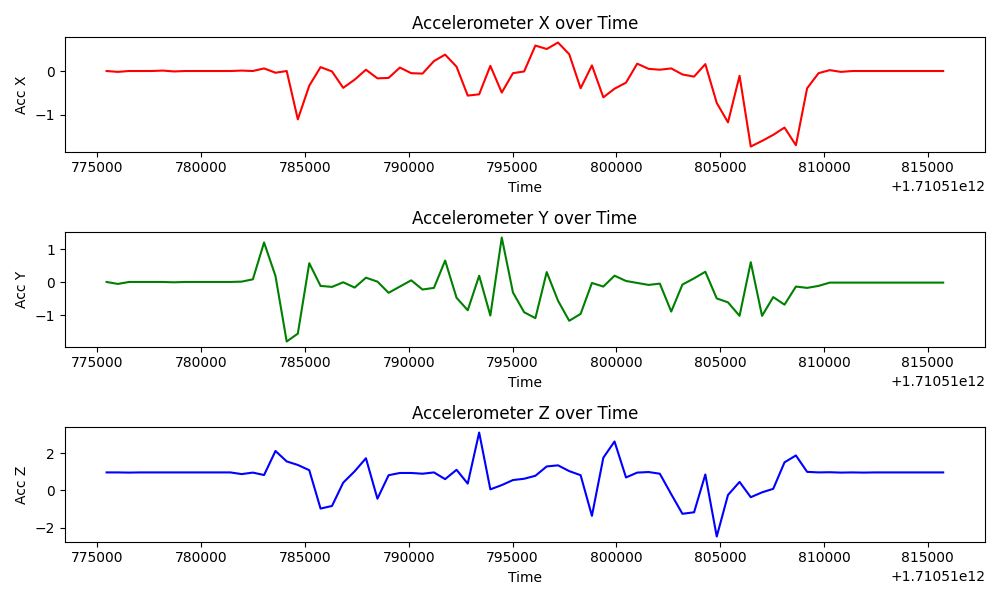
\includegraphics[width=0.7\textwidth]{scripts/shake1.png}
            \caption{Shake detection}
            \label{fig:shake1}
        \end{figure}

        \item
        \begin{verbatim}
if abs(acc_x) > 0.5 or abs(acc_y) > 0.5 or abs(acc_z) > 1.5:
    show = not show
        \end{verbatim}
    \end{enumerate}

    \item \textbf{Environment Sensing}
    \begin{enumerate}
        \item See Figure \ref{fig:environment1}. We attempted to affect the readings by covering the sensors with cloth (no noticeable effect) and blowing on them (temporarily spiking humidity and pressure readings, no noticeable temperature change).
        \begin{figure}
            \centering
            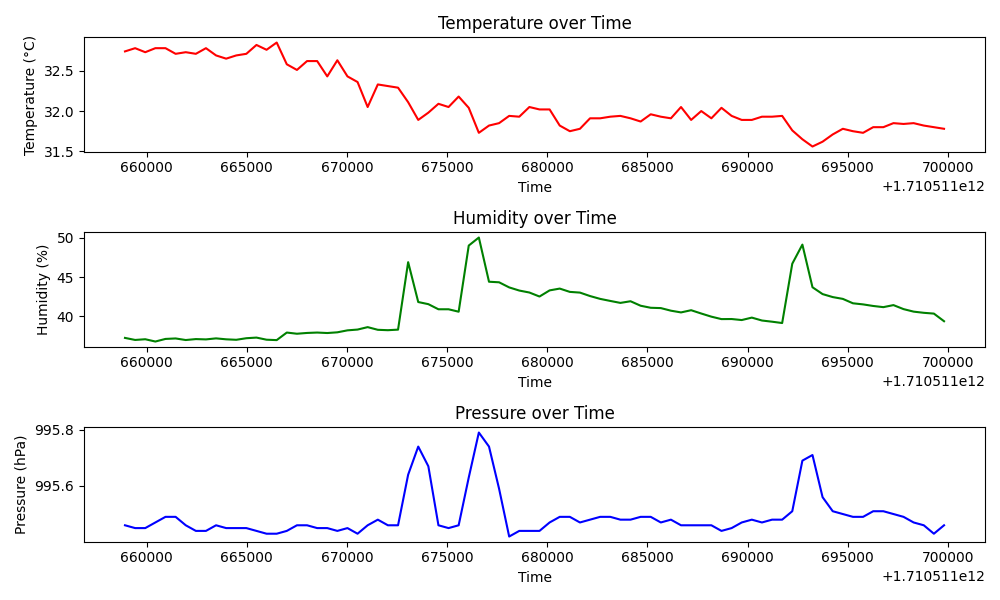
\includegraphics[width=0.7\textwidth]{scripts/environment1.png}
            \caption{Environment sensing}
            \label{fig:environment1}
        \end{figure}

        \item The temperature readings are not accurate, measurements were taken at room temperature. We assume that this is due to the heat that is emitted by the raspi itself, which felt warm to the touch.
    \end{enumerate}
\end{enumerate}

\end{document}
